\documentclass{article}
\usepackage{minted}
\usepackage{xcolor}
\usepackage{graphicx}
\graphicspath{{./images/}}
\usepackage{needspace}
\usepackage{xpatch}
\xpretocmd{\section}{\needspace{6\baselineskip}}{}{}
\definecolor{LightGray}{gray}{0.9}
\usemintedstyle{vs}
\title{Software Development Week 2}
\author{Nathan Le Brun}
\date{\today}
\begin{document}
    \maketitle
    \begin{flushleft}
        VSV Id: 107027
    \end{flushleft}
    \section{Functions}
        \subsection[1a]{Questions}
            \begin{enumerate}
                \item The names of the function parameters is \verb|$length| and \verb|$width|. A \verb|$| in front of the parameter name (\verb|$length|) denotes that it is a variable.
                \item The name of the variable that the function returns is \verb|$perimeterResult|.
                \item The line that calls the function is \verb|$perimeterResult = perimeterRectangle(4, 3);|.
                \item Due to PHP's loose type system and type-juggling system, both \verb|$length| and \verb|$height| can be of any type. For the function to execute correctly, \verb|$length| and \verb|$height| \textit{should} be of type \verb|int| or \verb|float|.
            \end{enumerate}
        \subsection{Area Function}
            \begin{minted}[breaklines, bgcolor=LightGray]{php}
<?php
  declare(strict_types = 1);
  
  function rectangle_area(int $width, int $height): int {
      return $width * $height;
  }
?>
            \end{minted}
    
    
        \subsection{Test Tables}
            \begin{tabular}{|c|c|c|c|}
                \hline
                \multicolumn{4}{|c|}{PerimeterRectangle} \\
                \hline
                Length & Width & Expected & Actual \\
                \hline
                4 & 3 & 14 & 14 \\
                \hline
                6&  3&  18& 18 \\
                \hline
                6&  6&  24& 24 \\
                \hline
            \end{tabular}
            \begin{tabular}{|c|c|c|c|}
                \hline
                \multicolumn{4}{|c|}{rectangle\_area} \\
                \hline
                Length & Width & Expected & Actual \\
                \hline
                4 & 3 & 12 & 12 \\
                \hline
                12 & 27 & 324 & 324 \\
                \hline
                6 & 6 & 24 & 36 \\
                \hline
            \end{tabular}
    \section{Strings}
        \subsection{String Functions}
            \begin{tabular}{|c|c|}
                \hline
                Function name & Description \\
                \hline
                \verb|strcasecomp()| & A case-insensitive comparison of two strings  \\
                \hline
                \verb|strcmp()| & A case-sensitive comparison of two strings \\
                \hline
                \verb|strtolower()| & Converts an entire string to lowercase \\
                \hline
                \verb|strtoupper()| & Converts an entire string to uppercase \\
                \hline
                \verb|strlen()| & Returns the amount of characters in the string (length) \\
                \hline
                \verb|ucfirst()| & Converts the first character in a string to uppercase \\
                \hline
                \verb|ucwords()| & Converts the first character of every word in a string to uppercase \\
                \hline
            \end{tabular}
        \subsection{Application of String Functions}
            \subsubsection{Code}
                \begin{minted}[breaklines, bgcolor=LightGray]{php}
<?php
  $test_sentence = "";
  if ($_SERVER["REQUEST_METHOD"] == "POST") {
    $test_sentence = test_input($_POST["test_sentence"]);
  }
  function test_input($data) {
    $data = trim($data);
    $data = stripslashes($data);
    $data = htmlspecialchars($data);
    return $data;
  }
?>
<form method="post" action="<?php echo htmlspecialchars($_SERVER["PHP_SELF"]);?>">
  Test Sentence:
  <input type="text" name="test_sentence" id="test_sentence">
  <br>
  <button type="submit">Submit</button>
</form>
<?php
  $perimeterResult = perimeterRectangle(4, 3);
  if ($test_sentence) {
    echo ucfirst($test_sentence) . "<br>";
    echo strlen($test_sentence) . "<br>";
    echo strtolower($test_sentence) . "<br>";
  }
?>
                \end{minted}
            \subsubsection{Output}    
                \begin{figure}[h]
                    \centering
                    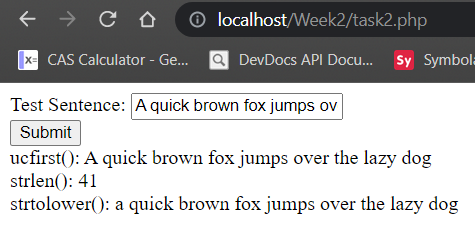
\includegraphics{StringCodeOutput}
                    \caption{The output of the code shown above}
                \end{figure}
\end{document}